\documentclass[12pt, letterpaper]{article}
\usepackage[hyphens]{url}
\setlength{\topmargin}{-1.75cm} \setlength{\textheight}{22.5cm}
\setlength{\oddsidemargin}{0.25cm}
\setlength{\evensidemargin}{0.25cm} \setlength{\textwidth}{16.2cm}
\renewcommand{\figurename}{Figure}
\usepackage{amssymb}
\usepackage{graphicx}
\usepackage{amsmath}
\usepackage[normalem]{ulem}
\usepackage{fontenc}
\usepackage{footnote}
\usepackage[breaklinks]{hyperref}
\usepackage{palatino, multicol, listings} % for multiple columns
\lstset{mathescape=true, basicstyle=\ttfamily,}

%\usepackage{pictex}
%% in the .pictex output of xfig, there is command \colo
%% however the old version of pictex may not define this
%% so we define color here as empty
%\def \color#1]#2{}

\begin{document}

\newcommand{\hide}[1]{}
\newcommand{\exercise}[1]{}
\newcommand{\future}[1]{}
\newcommand{\otherquestions}[1]{}
\newcommand{\set}[1]{\{#1\}}
\newcommand{\pg}[1]{{\tt #1}}
\newtheorem{definition}{Definition}
\newcommand{\emptyclause}{\Box}
\def\st{\bigskip\noindent}
\newcommand{\lplus}
{
   \stackrel{+}{\gets}
}

\newcommand{\fe}[1] {
  \begin{frame}
    #1
  \end{frame}}

\newcommand{\eoa}{ {\bf End} of algorithm}

\newcommand{\ft}[1] {\frametitle{#1}}

\newcommand{\ie}[1] {
  \begin{itemize}
    #1
  \end{itemize}
}

\newcommand{\ee}[1] {
  \begin{enumerate}
    #1
  \end{enumerate}\label{marker}
}
\newcommand{\blk}[2] {
  \begin{block}{#1}
    #2
  \end{block}
}

\newtheorem{collorary}{Corollary}
\newtheorem{proposition}{Proposition}
\newtheorem{invariant}{Invariant}
\newtheorem{property}{Property}
\newtheorem{claim}{Claim}
\newtheorem{example}{Example}


\title{${\cal ELPS}$ manual}
\date{\today}
\maketitle
\tableofcontents
\pagebreak


\section{System installation}

\st For using the system, you need to have the following installed:
\begin{enumerate}
\item Java Runtime Environment (JRE): \\
{\scriptsize
\url{http://www.oracle.com/technetwork/java/javase/downloads/index.html}
}.\\
The system was tested on Java versions 1.6.0\_37 and 1.7.0\_25.
\item The ELPS binary file: \\ 
{\scriptsize
\url{https://github.com/iensen/elps/blob/master/elps.jar?raw=true}
}.

\item Clingo (version 4.2.1 or later):\\ {\scriptsize
 \url{http://sourceforge.net/projects/potassco/files/clingo/4.2.1}}


\end{enumerate}

Be sure the PATH system variable includes the directory where the clingo executable is located. For instructions on how to view/modify the PATH system variable, see either of the following links:\\
{\scriptsize
\url{http://www.java.com/en/download/help/path.xml}\\
\url{http://www.cyberciti.biz/faq/appleosx-bash-unix-change-set-path-environment-variable/}\\
}
To check if clingo is installed correctly, run the command  \texttt{clingo -v}. See figure \ref{fig:clingo_solver_check} for the expected output.

\begin{figure}[h!]
\centering
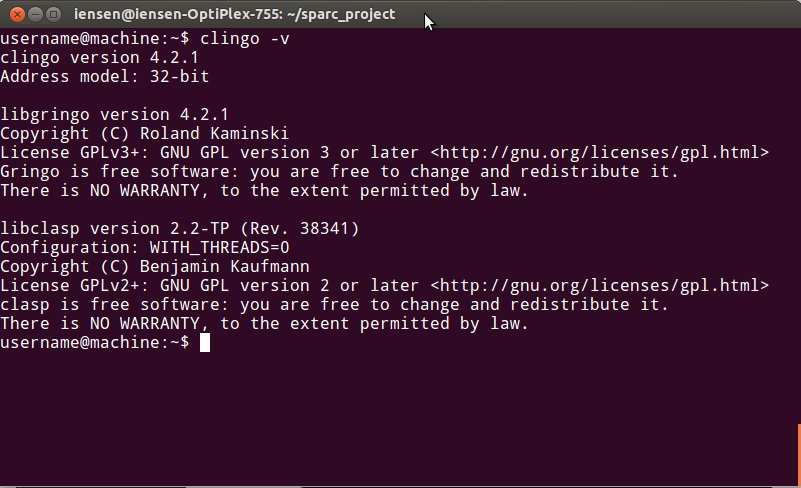
\includegraphics[width=0.9\textwidth]{clingo_version.jpg}
\caption{Checking the version of Clingo solver}
\label{fig:clingo_solver_check}
\end{figure}

\section{System usage}

To demonstrate the usage of the system we will use the program  below described in \cite{epist}.
\begin{verbatim}
sorts
#student = {mike,mary,ann}.

predicates

eligible(#student).
highGPA(#student).
fairGPA(#student).
minority(#student).
interview(#student).

rules
eligible(X):- highGPA(X).
eligible(X):- minority(X), fairGPA(X).
-eligible(X):- -fairGPA(X), -highGPA(X).
interview(X):- not K$ eligible(X), not K$ -eligible(X).

% data
fairGPA(mike) | highGPA(mike).
highGPA(mary).
\end{verbatim}

To run  ${\cal ELPS}$ solver  on the program above, 
we change current directory to a directory having the file \texttt{program.sp} with the program written in it, and the downloaded file \texttt{elps.jar}.  Then, we run the command:
\begin{verbatim}

> java -jar elps.jar program.sp
ELPS V1.04
program translated
World View 1 out of 1:
{eligible(mary), student(mary), student(ann), student(mike), 
interview(mike), interview(ann), highGPA(mary), fairGPA(mike)}

{eligible(mary), student(mary), student(ann), student(mike), 
interview(mike), interview(ann), highGPA(mike), highGPA(mary), 
eligible(mike)}


\end{verbatim}
The program has a single world view, which contains \texttt{interview(mike)} in both belief sets.




\section{Syntax Description}

\subsection{Directives}
Directives should be written before sort definitions, at the very beginning of a program.
${\cal ELPS}$ allows two types of directives:
\subsection*{\#maxint}
Directive \#maxint specifies the maximum nonnegative number that could be used in arithmetic calculations.
For example,
\begin{verbatim}
 #maxint=15.
\end{verbatim}
\st limits integers to [0,15].
\subsection*{\#const}
Directive \#const allows one to define constant values. The syntax is:

\begin{verbatim}
   #const constantName = constantValue.
\end{verbatim}      
\st where $constantName$  must begin with a lowercase letter and may be composed of letters, underscores and digits,
 and $constantValue$ is either a nonnegative number or the name of another constant defined before it.  


\subsection{Sort definitions}\label{ss}

This section starts with a keyword $sorts$ followed by a collection of sort definitions of the form:

\begin{equation*}
  sort\_name=sort\_expression.
\end{equation*}
\textit{sort\_name} is an identifier preceeded by the pound sign (\#).
\textit{sort\_expression}  on the right hand side denotes a collection of strings called  $a~sort$. We divide all the sorts into \textit{basic sorts} and \textit{non-basic sorts}. 

\st \textit{Basic sorts} are defined as named collections of numbers and \textit{identifiers}, i.e, strings consisting of
\begin{itemize}
 \item letters: $\{a,b,c,d,...,z,A,B,C,D,...,Z\}$
 \item digits: $\{0,1,2,...,9\}$
 \item underscore: $\_$
\end{itemize}
and starting with a lowercase letter.

A \textit{non-basic sort} also contains at least one \textit{record} of the form $id(\alpha_1,\dots, \alpha_n)$ where $id$ is an identifier and 
$\alpha_1, \dots, \alpha_n$ are either identifiers, numbers or records. 


\st We define sorts by means of expressions (in what follows sometimes referred to as statements) of six types:

\begin{enumerate}

\item
\textbf{numeric range}  of the form
\begin{equation*}
n_1..n_2
\end{equation*}

where $n_1$ and $n_2$ are non-negative integer numbers such that $n_1 \le n_2$. The expression defines the set 
of sequential numbers $\{n_1, n_1+1, \dots, n_2\}$.

\textit{Example:}

\begin{verbatim}
 #sort1=1..3.
\end{verbatim}
\texttt{\#sort1} consists of numbers $\{1,2,3\}$.


\item \textbf{identifier range}  of the form

\begin{equation*}
  id_1..id_2
\end{equation*}
where $id_1$ and $id_2$ are identifiers, 
$id_1$ is lexicographically \footnote{ The system default encoding is used for  ordering of individual characters} smaller than or equal to  $id_2$, and the length of $id_1$ is less than or equal to the length of $id_2$. That is,  $id_1 \leq id_2$ and $|id_1| \leq |id_2|$.
The expression defines the set of strings  $\{s: id_1\leq s \leq id_2 \land |id_1|\leq |s| \leq |id_2|\}$.



\textit{Example:}

\begin{verbatim}
 #sort1=a..f.
\end{verbatim}

\texttt{\#sort1} consists of letters $\{a,b,c,d,e,f\}$.

\item \textbf{set of ground terms}  of the form


\begin{equation*}
\{t_1,..,,t_n\}
\end{equation*}

The expression denotes a set of \textit{ground terms} $\{t_1,...,t_n\}$, defined as follows:
\begin{itemize}
 \item numbers and identifiers are ground terms;
 \item If $f$ is an identifier and $\alpha_1, \dots, \alpha_n$ are ground terms, then $f(\alpha_1,\dots, \alpha_n)$ is a ground term.
\end{itemize}
\textit{Example} : 
\begin{verbatim}
 #sort1={f(a),a,b,2}.
\end{verbatim}






\item \textbf{set of records} of the form

\begin{equation*}
f(sort\_name_1(var_1),..., sort\_name_n(var_n)):
                                     condition(var_1,...,var_n)
\end{equation*}
where $f$ is an identifier, for $ 1\leq i\leq m$ $sort\_name_i$ occurs in one of the preceeding sort definitions and  the condition on variables $var_1,...,var_n$ (written as $condition(var_1,...,var_n)$) is defined as follows:
\begin{itemize}
\item if $var_i$ and $var_j$ occur in the sequence  $var_1,...,var_n$ and $\odot$ is an element of $\{>,<,\le,\ge\}$, then $var_i \odot var_j$ is a condition on   $var_1,...,var_n$.
\item if $\mathcal{C}_1$ and $\mathcal{C}_2$ are both conditions on  $var_1,...,var_n$, and $\oplus$ is an element of  $\{\cup,\cap\}$, then
$(\mathcal{C}_1 \oplus \mathcal{C}_2)$ is a condition on  $var_1,...,var_n$.
\item if $\mathcal{C}$ is a  condition on  $var_1,...,var_n$, then $not(\mathcal{C})$ is also a condition on  $var_1,...,var_n$.
\end{itemize}


Variables $var_1,...,var_n$ occurring in parenthesis after sort names are optional as well as the condition :$condition(var_1,...,var_n)$.

If a condition contains a subcondition $var_i~\odot~var_j$,  then the sorts  $sortname_i$ and  $sortname_j$
must be defined by basic statements (the definition of a basic statement is given below after the definition of a concatenation statement).

The expression defines a collection of ground terms 
\\ $\{f(t_1,\dots,t_n):  t_1 \in s_i \land \dots \land t_n \in s_n \land (condition(X_1,\dots, X_n)|_{X_1 = t_1,\dots,X_n = t_n})\}$

\textit{Example}
\begin{verbatim}
 #s=1..2.
 #sf=f(s(X),s(Y),s(Z)): (X=Y or Y=Z). 
\end{verbatim}

The sort \texttt{\#sf} consists of records $\{f(1,1,2),f(1,1,1),f(2,1,1)\}$
 \item \textbf{set-theoretic expression}  in one of the following forms
\begin{itemize}
\item $\#sort\_name$  
\item an expression of the form (3), denoting a set of ground terms
\item an expression of the form (4), denoting a set of records
\item $(S_1 \bigtriangledown S_2)$, where $\bigtriangledown \in \{+,-,*\}$ and both $S_1$ and $S_2$ are set theoretic expressions
\end{itemize}

$\#sort\_name$ must be a name of a sort occurring in one of the preceeding sort definitions. 
The operations $+$ $*$ and $-$ stand for union, intersection and difference correspondingly.
\pagebreak

\textit{Example} : 
\begin{verbatim}
 #sort1={a,b,2}.
 #sort2={1,2,3} + {a,b,f(c)} + f(#sort1).
\end{verbatim}
 \texttt{\#sort2} consists of ground terms $\{1,2,3,a,b,f(c),f(a),f(b),f(2)\}$.
\item \textbf{concatenation} of the form
\begin{equation*}
 [b\_stmt_1] ... [b\_stmt_n]
\end{equation*}

$b\_stmt_1, \dots, b\_stmt_n$ must be \textit{basic statements}, defined as follows:


\begin{itemize}
 \item statements of the forms (1)-(3) are basic
 \item statement $S$ of the form (5) is basic if:
 \begin{itemize}
 \item it does not contain sort expressions of the form (4), denoting sets of records
  \item none of curly brackets occurring in $S$ contains a record
  \item all sorts occurring in $S$ are defined by basic statements 
 \end{itemize}
\end{itemize}
Note that basic statement can only define a basic sort.

\textit{Example\footnote{We allow a shorthand `b` for singleton  set \{b\}}.:}

\begin{verbatim}
 #sort1=[b][1..100].
\end{verbatim}

\texttt{sort1} consists of identifiers $\{b1,b2,\dots, b100\}$.

\end{enumerate}

\subsection{Predicate Declarations}

\noindent  The second part of a  ${\cal ELPS}$ program starts with the keyword
\st
$predicates$

\st and is followed by statements of the form

\begin{equation*}
pred\_symbol(\#sortName_1,\dots,\#sortName_n)
\end{equation*}
\st

Where $pred\_symbol$ is an identifier (in what follows referred to as a predicate symbol) and  $\#sortName_1$,\dots,$\#sortName_n$ are sorts defined in sort definitions section of the program.



Multiple declarations containing the same predicate symbol are not allowed.
0-arity predicates must be declared as $pred\_symbol()$.
\st For any sort name $\#s$, the system includes declaration  $\#s(\#s)$ automatically. 

\subsection{Program Rules}


\st The third part of a ${\cal ELPS}$ program starts with the keyword \textit{rules} followed by  rules of the form

\begin{equation}
   \ell_0 | \ell_1 \dots |\ell_n \gets  g_1, \ldots, g_m, not~g_{m+1} \ldots not~g_{k}.
\end{equation}
where  $k\ge 0$, $m \ge 0, k\ge  m$,
each $l_i$ is a literal and each $g_i$ is  either an extended literal(i.e, a literal possibly preceeded by $not$) or a subjective literal. Subjective literals can be in one of the forms $K\$\ell$,$M\$\ell$, $not~ K\$\ell$, or $not~M\$\ell$, where $\ell$ is a literal.
 
Literals occurring in the heads of the rules must not be formed by predicate symbols
occurring as sort names in sort definitions. In addition, rules must not contain \textit{unrestricted variables}.

\begin{definition}(Unrestricted Variable)
 A variable occurrung in a rule of a ${\cal SPARC}$ program is called unrestriced if all its occurrences in the rule either belong to some relational atoms of the form 
$term1$ \textbf{rel} $term2$ (where \textbf{rel} $\in  \{>,>=,<,<=,=,!=$\})  and/or  some term appearing in a head of a choice or aggregate element. 
\end{definition}
\begin{example}
\em{
 Consider the following ${\cal ELPS}$ program:
\begin{verbatim}
sorts
#s={f(a),b}.
predicates
p(#s).
rules
p(f(X)):-Y<2,2=Z,F>3,#count{Q:Q<W,p(W),T<2},p(Y).
\end{verbatim}
Variables F,T,Z,Q are unrestricted.
}  
\end{example}

 

\section{Typechecking}
If no syntax errors are found, a static check of the program is performed. Any type-related problems found during this check 
will be output as type errors
\subsection{Type errors}
Type errors are considered as serious issues which make it  impossible to compile and execute the program.
Type errors can occur in all four sections of a ${\cal ELPS}$ program.
\subsubsection{Sort definition errors}
The following are possible causes of a sort definition error  that will result in a type error  message from ELPS:
\begin{enumerate}
\item  A set-theoretic expression (statement 5 in section \ref{ss}) containing a sort name that has not been defined.

\textit{Example:}
\begin{verbatim}
 sorts
 #s={a}.
 #s2=#s1-#s.
\end{verbatim}

\item  Declaring a sort more than once.

\textit{Example:}
\begin{verbatim}
 sorts
 #s={a}.
 #s={b}.
\end{verbatim}

\item An identifier range $id_1..id_2$ (statement 2 in section \ref{ss}) where $id_1$ is greater than $id_2$.

\textit{Example:}
\begin{verbatim}
 sorts
 #s=zbc..cbz.
\end{verbatim}

\item A numeric range $n_1..n_2$ (statement 1 in section \ref{ss}) where  $n_1$ is greater than $n_2$.

\textit{Example:}
\begin{verbatim}
 sorts
 #s=100500..1.
\end{verbatim}


\item A numeric range (statement 1 in section \ref{ss}) $n_1..n_2$ that  contains an undefined constant.

\textit{Example:}
\begin{verbatim}
 #const n1=5.
 sorts
 #s=n1..n2.
\end{verbatim}

\item An identifier range $id_1..id_2$ (statement 2 in section \ref{ss}) where  the length of $id_1$ is greater than the length of $id_2$. 


\textit{Example:}
\begin{verbatim}
 sorts
 #s=abc..a.
\end{verbatim}

\item A concatenation (statement  6 in section \ref{ss}) that contains a non-basic sort.

\textit{Example:}
\begin{verbatim}
 sorts
 #s={f(a)}.
 #sc=[a][#s].
\end{verbatim}



\item A record definition (statement 5 in section \ref{ss}) that contains an undefined sort.

\textit{Example:}
\begin{verbatim}
 sorts
 #s=1..2.
 #fs=f(s,s2).
\end{verbatim}



\item A record definition  (statement 5 in section \ref{ss}) that contains a condition with relation $>,<,\geq,\leq$ such that the
   corresponding sorts are not defined by  basic statements.

\textit{Example:}
\begin{verbatim}
#s={a,b}.
#s1=f(#s). 
#s2=g(s1(X),s2(Y)):X>Y.
\end{verbatim}

\item  A variable that is used more than once in a record definition (statement  5 in section \ref{ss}).

\textit{Example:}

\begin{verbatim}
 sorts
 #s1={a}.
 #s=f(#s1(X),#s1(X)):(X!=X).
\end{verbatim}
\item A sort that contains an empty collection of ground terms.

\textit{Example}
\begin{verbatim}
 sorts
 #s1={a,b,c}
 #s=#s1-{a,b,c}.
\end{verbatim}
\end{enumerate}
\subsubsection{Predicate declarations errors}

\begin{enumerate}
\item A predicate with the same name is defined more than once.

\textit{Example:}
\begin{verbatim}
 sorts
 #s={a}.
 predicates
 p(#s).
 p(#s,#s).
\end{verbatim}
\item A predicate declaration contains an undefined sort.

\textit{Example:}
\begin{verbatim}
 sorts
 #s={a}.
 predicates
 p(#ss).
\end{verbatim}
\end{enumerate}
\subsubsection{Program rules errors}

In program rules we first check each atom of the form $p(t_1,\dots,t_n)$ and each term occurring in the program $\Pi$ for satisfying
the definitions of program atom and program term correspondingly\cite{sparc}. Moreover, we check that no sort occurs in a head of a rule of $\Pi$.

\bibliography{mybib}
\bibliographystyle{plain}
\end{document}

